\chapter{Structuurbiologie van eiwitten}\label{ch:b3:structural-biology}

Max Perutz begon in 1937 aan de structuur van hemoglobine en
publiceerde haar in 1960: tweeëntwintig jaar om, met een \omterm{def:b3:structural-biology:methods}{resolutie} van
een halve nanometer, te zien hoe vier ketens van honderdvijftig
aminozuren zich om vier hemen vouwen. Een hemoglobinemolecuul vouwt
zichzelf in enkele milliseconden. Tussen die twee feiten ligt het
onderwerp van dit hoofdstuk: wat de vorm van een eiwit is, waarom een
keten aminozuren de ene vorm heeft en niet de andere, hoe zij die vorm
zo snel vindt tussen een astronomisch aantal alternatieven, wat er
misgaat wanneer dat niet lukt, hoe de vormen worden gezien --- met
röntgenstraling, met magnetische resonantie, met elektronen en
tegenwoordig met de computer --- en hoe een eiwit tussen vormen beweegt
om zijn werk te doen, met de omschakeling van hemoglobine tussen een
gespannen en een ontspannen vorm als het model voor elk allosterisch
eiwit sindsdien.

\section{Wat de structuur van een eiwit is}

\begin{definition}[Structuurniveaus]\label{def:b3:structural-biology:levels}
\index{secundaire structuur}\index{alfahelix}\index{bèta-plaat}\index{tertiaire structuur}\index{domein}\index{vouwing}
De \emph{primaire structuur} is de volgorde van de residuen. De
\emph{secundaire structuur} is de plaatselijke regelmatige conformatie
van de ruggengraat, gestabiliseerd door waterstofbruggen tussen
carbonylen en amiden van de ruggengraat: de \emph{$\alpha$-helix}, een
rechtsdraaiende spiraal van $3.6$ residuen per winding die
\qty{0.15}{nm} per residu stijgt (\qty{0.54}{nm} per winding), waarbij
elk carbonyl aan het amide vier residuen verder is gebonden; en de
\emph{$\beta$-plaat}, waarin gestrekte strengen naast elkaar liggen,
parallel of antiparallel, aan hun buren gebonden, met de zijketens
afwisselend boven en onder de plaat. De \emph{tertiaire structuur} is
de vouwing van een hele keten in drie dimensies; een compacte,
zelfstandig vouwende eenheid van \numrange{50}{250} residuen daarbinnen
is een \emph{domein}, en de schikking van de secundaire elementen van
een domein is zijn \emph{vouwing}. De \emph{quaternaire structuur} is
de samenstelling van verscheidene ketens: de $\alpha_{2}\beta_{2}$ van
hemoglobine. Ongeveer \num{1300} vouwingen dekken alle bekende domeinen,
en enkele tientallen daarvan --- de Rossmann-vouwing, het TIM-vat, de
immunoglobulinevouwing --- een groot deel van alle eiwitten: de natuur
hergebruikt vouwingen en varieert hun sequenties.
\end{definition}

\begin{omfigure}
\begin{tikzpicture}
\begin{axis}[
  width=6.4cm, height=6.4cm,
  xmin=-180, xmax=180, ymin=-180, ymax=180,
  xlabel={$\phi$ (graden)}, ylabel={$\psi$ (graden)},
  xlabel style={font=\small}, ylabel style={font=\small},
  tick label style={font=\scriptsize}, xtick={-180,-90,0,90,180}, ytick={-180,-90,0,90,180},
  axis lines=box, grid=major, grid style={gray!25},
  clip=false,
]
% beta region
\fill[omDef!30] (axis cs:-180,90) rectangle (axis cs:-45,180);
\fill[omDef!30] (axis cs:-180,-180) rectangle (axis cs:-45,-150);
\node[font=\scriptsize, omDef!60!black] at (axis cs:-112,165) {$\beta$-strengen};
% alpha R region
\fill[omThm!30] (axis cs:-160,-70) rectangle (axis cs:-45,0);
\node[font=\scriptsize, omThm!70!black] at (axis cs:-105,-58) {rechtsdraaiende $\alpha$};
% alpha L region
\fill[omMeth!30] (axis cs:45,0) rectangle (axis cs:100,80);
\node[font=\scriptsize, omMeth!60!black, align=center] at (axis cs:72,40) {links-\\draaiend};
\addplot[only marks, mark=*, mark size=1pt, black] coordinates {(-57,-47)};
\node[font=\scriptsize, anchor=south west] at (axis cs:-52,-44) {$\alpha$: $(-57,-47)$};
\addplot[only marks, mark=*, mark size=1pt, black] coordinates {(-139,135)};
\node[font=\scriptsize, anchor=west] at (axis cs:-134,135) {antiparallelle $\beta$};
\end{axis}
\node[align=left, font=\scriptsize, anchor=west] at (7.0,3.0) {De twee torsiehoeken van de ruggengraat\\van elk residu, $\phi$ (om N--C$_\alpha$) en $\psi$ (om\\C$_\alpha$--C), zijn door sterische botsingen\\beperkt tot de gekleurde gebieden. Een helix zet elk\\residu op één punt; een streng vlak bij een ander.\\Glycine, zonder zijketen, reikt verder;\\proline, met zijn ring, ligt vast bij $\phi = -60$.};
\end{tikzpicture}

{\small De ramachandranplot. De gekleurde gebieden zijn de sterisch
toegestane combinaties van de hoeken $\phi$ en $\psi$ van de
ruggengraat; de rechtsdraaiende $\alpha$-helix en de $\beta$-streng
komen elk met een klein gebied overeen, en de meeste residuen van een
gevouwen eiwit vallen in een van beide.}
\end{omfigure}

\begin{proposition}[Wat een vouwing bijeenhoudt]\label{prop:b3:structural-biology:forces}
\index{hydrofoob effect}\index{marginale stabiliteit}
Een gevouwen eiwit wordt gestabiliseerd door het \emph{\omterm{prop:b3:structural-biology:forces}{hydrofobe
effect}} --- apolaire zijketens in een kern weg van het water begraven,
wat de watermoleculen vrijmaakt die er anders omheen geordend zouden
staan --- door de waterstofbruggen van de \omterm{def:b3:structural-biology:levels}{secundaire structuur} en van
begraven polaire groepen, door vanderwaalspakking van een kern die zo
dicht is als een kristal, door incidentele zoutbruggen en, bij
uitgescheiden eiwitten, door zwavelbruggen. Het \omterm{prop:b3:structural-biology:forces}{hydrofobe effect} levert
het grootste deel van de drijvende kracht; de waterstofbruggen betalen
grotendeels zichzelf terug (een ruggengraat die in de ongevouwen
toestand aan water is gebonden, is in de gevouwen toestand aan zichzelf
gebonden) en bepalen in plaats daarvan \emph{welke} \omterm{def:b3:structural-biology:levels}{vouwing} ontstaat.
De netto vrije energie van de \omterm{def:b3:structural-biology:levels}{vouwing} is klein,
$\Delta G \approx -20$ tot \qty{-60}{kJ/mol} --- de sterkte van een
handvol waterstofbruggen voor een molecuul met honderden --- omdat het
verlies aan conformatie-entropie bij het vouwen de winst aan enthalpie
bijna opheft. Eiwitten zijn \emph{marginaal stabiel}: enkele graden,
een verandering van pH of één enkele mutatie in de kern kan ze
ontvouwen, en juist die marginaliteit laat ze bewegen.
\end{proposition}

\begin{proof}[Bewijsmateriaal]
Anfinsen (1961) ontvouwde ribonuclease~A met ureum en een
reductiemiddel, waarbij zijn vier zwavelbruggen werden verbroken en
zijn werking verdween; toen hij beide verwijderde, vouwde het enzym
zich terug, vormde het de juiste vier van de $105$ mogelijke
zwavelbrugparen opnieuw, en kreeg het zijn volle werking terug. Er was
geen matrijs, geen enzym en geen informatie buiten de sequentie
aanwezig: de natieve structuur is de thermodynamisch stabielste
toestand die de keten kan bereiken, en de sequentie legt haar vast. De
zwavelbruggen opnieuw oxideren terwijl de keten nog in ureum zat gaf
een door elkaar gehusseld mengsel met \qty{1}{\%} werking, dat zich
daarna, als het mocht vouwen, tot de natieve vorm ontwarde: de keten
vindt het minimum zelf.
\end{proof}

\section{Hoe een keten haar vouwing vindt}

\begin{theorem}[De paradox van Levinthal]\label{thm:b3:structural-biology:levinthal}
\index{paradox van Levinthal}\index{vouwtrechter}
Als elk van de $n$ residuen van een eiwit onafhankelijk $k$
conformaties van de ruggengraat kon aannemen, zou de keten $k^{n}$
conformaties hebben. Met $k = 3$ en $n = 100$ is dat $3^{100} \approx
5\times 10^{47}$; ze bemonsteren met één per picoseconde ($10^{12}$ per
seconde) zou $5\times 10^{35}$ seconden kosten, ongeveer $10^{28}$
jaar. Eiwitten van deze grootte vouwen zich in milliseconden tot
seconden. Het vouwen is dus geen willekeurige zoektocht door de
conformaties: het energieoppervlak is een \emph{trechter}, waarin
vrijwel elke gedeeltelijke conformatie naar de natieve toestand neigt,
en de keten daalt af met plaatselijke zetten die elk gemiddeld
bergafwaarts gaan.
\end{theorem}
\begin{proof}
De telling is het vermenigvuldigingsbeginsel; de tijd is de telling
gedeeld door de bemonsteringssnelheid,
$5\times 10^{47}/10^{12} = 5\times
10^{35}$ s, en een jaar is $3\times 10^{7}$ s. De gevolgtrekking is de
contrapositie: een willekeurige zoektocht van die omvang is in de
waargenomen tijd onmogelijk, dus is de zoektocht niet willekeurig. Wat
haar niet-willekeurig maakt is dat een interactie die in het ene deel
van de keten wordt gevormd blijft bestaan terwijl andere ontstaan (de
hydrofobe ineenstorting en de vorming van helices gebeuren in
microseconden en verkleinen de te doorzoeken ruimte), en dat
gedeeltelijk juiste structuren gemiddeld lager in energie liggen dan
verkeerde, zodat de afdaling wordt geleid --- een trechter en niet een
golfbaan met één enkele hole.
\end{proof}

\begin{omfigure}
\begin{tikzpicture}[every node/.style={font=\scriptsize}, >=stealth]
  % funnel outline
  \draw[very thick, omDef] (-4,3) .. controls (-3.2,1.5) and (-1.2,0.2) .. (-0.35,-1.2) -- (-0.35,-1.6);
  \draw[very thick, omDef] (4,3) .. controls (3.2,1.5) and (1.2,0.2) .. (0.35,-1.2) -- (0.35,-1.6);
  \draw[very thick, omDef] (-0.35,-1.6) -- (0.35,-1.6);
  % rugged inner lines
  \draw[omDef!60, thick] (-3.3,2.6) .. controls (-2.9,2.2) and (-2.6,2.6) .. (-2.2,2.0) .. controls (-1.9,1.5) and (-1.7,1.9) .. (-1.4,1.2) .. controls (-1.1,0.7) and (-0.9,0.9) .. (-0.6,0.2);
  \draw[omDef!60, thick] (3.3,2.6) .. controls (2.9,2.1) and (2.5,2.5) .. (2.1,1.8) .. controls (1.8,1.3) and (1.5,1.6) .. (1.2,1.0) .. controls (1.0,0.6) and (0.8,0.8) .. (0.6,0.2);
  % axes
  \draw[->] (-5.9,-1.8) -- (-5.9,3.2) node[above, align=center] {vrije\\energie};
  \draw[<->] (-3.9,3.85) -- (3.9,3.85) node[midway, above] {conformatie-entropie (breedte van het ensemble)};
  % labels
  \node[above] at (0,3.05) {ongevouwen keten: veel conformaties, hoge energie};
  \node[right, align=left] at (3.3,1.4) {plaatselijke vallen: deels\\verkeerd gevouwen tussenvormen};
  \node[left, align=right] at (-3.3,1.4) {snelle ineenstorting en\\secundaire structuur};
  \node[below] at (0,-1.7) {natieve toestand: één conformatie, laagste energie};
  \draw[->, thick, omThm] (-2.8,2.4) .. controls (-2.0,1.2) and (-0.8,0.5) .. (-0.15,-1.3);
  \node[omThm, left] at (-1.5,-0.5) {een vouwtraject};
\end{tikzpicture}

{\small De \omterm{thm:b3:structural-biology:levinthal}{vouwtrechter}. De vrije energie daalt en het aantal
beschikbare conformaties krimpt naarmate de keten de natieve toestand
nadert; de wanden zijn ruw, zodat een keten in een deels verkeerd
gevouwen tussenvorm gevangen kan raken, maar de algemene helling voert
haar in milliseconden omlaag.}
\end{omfigure}

\begin{definition}[Chaperonnes]\label{def:b3:structural-biology:chaperones}
\index{chaperonne}\index{Hsp70}\index{chaperonine}\index{GroEL}
Een \emph{moleculaire chaperonne} is een eiwit dat het vouwen van
andere eiwitten bijstaat zonder er deel van te worden of informatie
over de \omterm{def:b3:structural-biology:levels}{vouwing} te leveren: zij verhindert de samenklontering die in
het drukke cytoplasma met het vouwen wedijvert. \emph{Hsp70} bindt
blootliggende hydrofobe segmenten van ontluikende of ongevouwen ketens
en laat ze bij ATP-hydrolyse los voor een nieuwe poging; de
\emph{chaperonine} GroEL (Hsp60 in mitochondriën, TRiC in het
eukaryote cytosol) is een dubbel vat van veertien subeenheden waarvan
de centrale holte, afgesloten door GroES, één enkele keten van
hoogstens \qty{60}{kDa} ongeveer tien seconden in afzondering opsluit
--- een anfinsenkooi --- en haar daarna uitwerpt, gevouwen of niet, om
het opnieuw te proberen. Ongeveer een tiende van de nieuw gemaakte
bacteriële eiwitten gaat door GroEL, en een cel waarvan de chaperonnes
worden overvraagd --- door hitte, en daarom zijn de meeste
\emph{hitteschokeiwitten} die door een temperatuurstijging worden
aangezet --- loopt vol klonters.
\end{definition}

\begin{definition}[Amyloïd]\label{def:b3:structural-biology:amyloid}
\index{amyloïd}\index{cross-bèta}\index{prion}\index{vouwingsziekte}
\emph{Amyloïd} is een geordende klontering van eiwit waarin de ketens
zich opstapelen tot onvertakte vezels van \qtyrange{5}{10}{nm} breed,
waarbij de strengen van elke keten loodrecht op de vezelas lopen en met
waterstofbruggen aan de strengen van de volgende keten zijn gebonden
--- de \emph{cross-$\beta$}-structuur, dezelfde voor welk eiwit ook.
Vrijwel elk eiwit kan haar onder destabiliserende omstandigheden
vormen; bij de \emph{vouwingsziekten} doen bepaalde eiwitten dat in
het lichaam: amyloïd-$\beta$ en tau bij de ziekte van Alzheimer,
$\alpha$-synucleïne bij die van Parkinson, huntingtine, transthyretine,
eilandjesamyloïd bij diabetes type~2. Een \emph{prion} is een amyloïd
dat zich voortplant: de verkeerd gevouwen vorm van het prioneiwit PrP
zet bij aanraking de normale vorm om in meer van zichzelf, zodat de
``besmetting'' geen nucleïnezuur draagt maar alleen een vorm --- het
mechanisme van scrapie, van boviene spongiforme encefalopathie en van
de ziekte van Creutzfeldt--Jakob, door Prusiner vanaf 1982 tegen lange
weerstand in vastgesteld.
\end{definition}

\begin{omfigure}
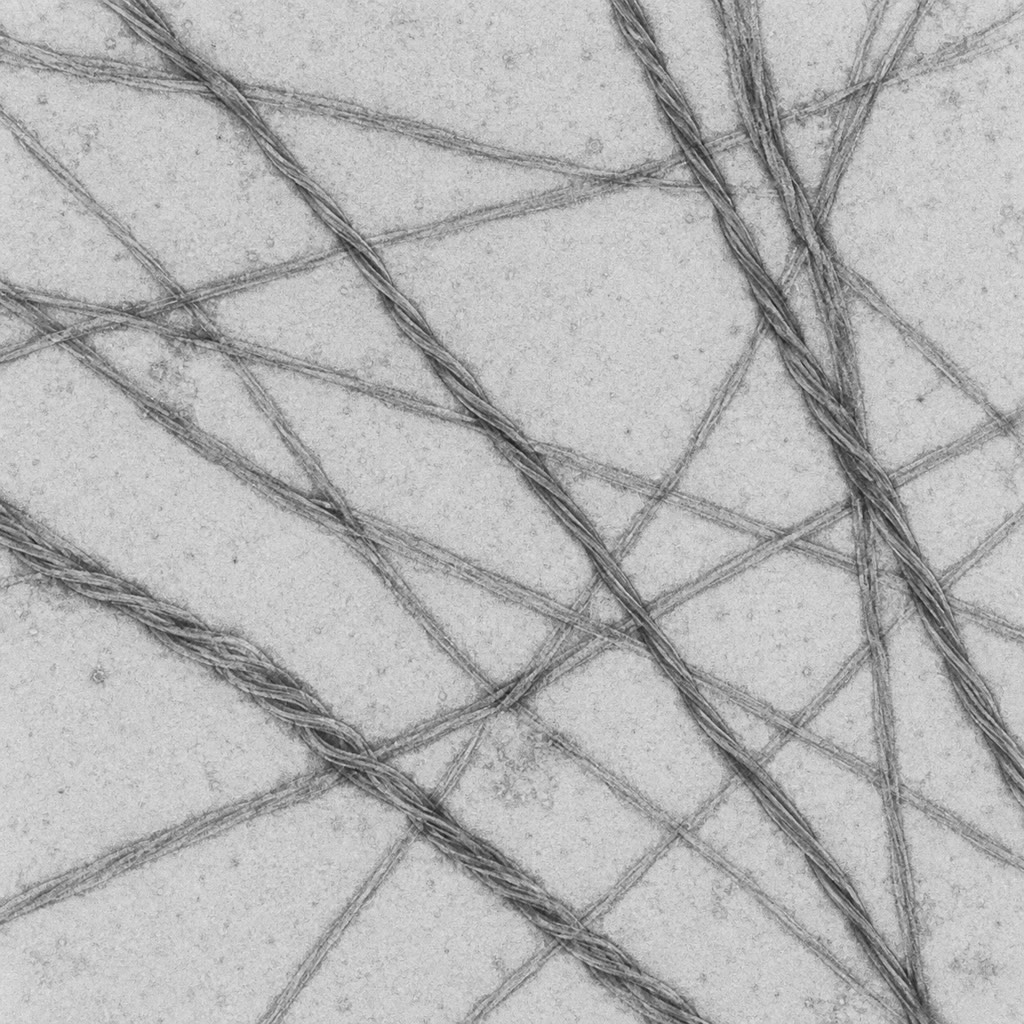
\includegraphics[width=0.36\linewidth]{images/book5/ai/b5-07-amyloid-fibrils.jpg}\hspace{0.04\linewidth}
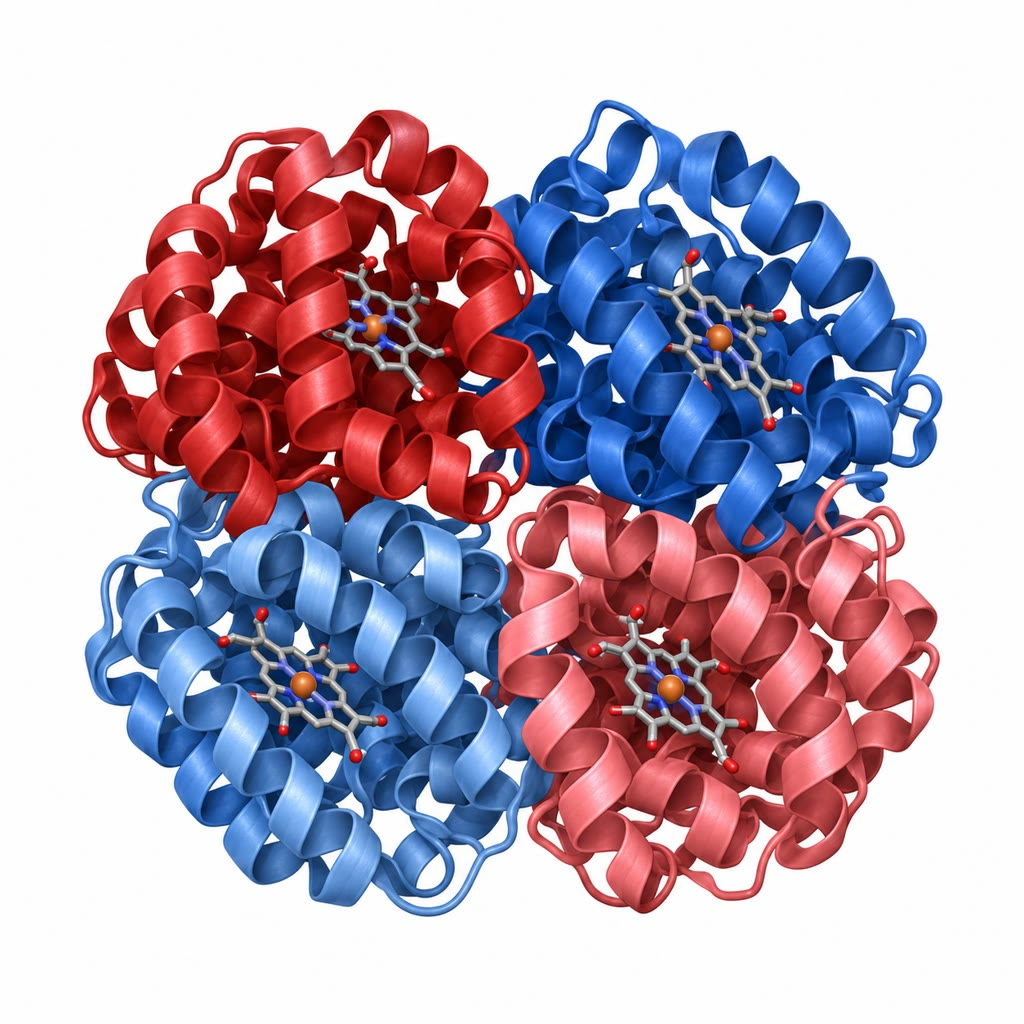
\includegraphics[width=0.36\linewidth]{images/book5/ai/b5-07-haemoglobin-model.jpg}

{\small Links: amyloïdvezels in de elektronenmicroscoop --- recht,
onvertakt, soms gedraaid, en van bouw gelijk uit welk eiwit zij ook
bestaan. Rechts: het hemoglobinetetrameer, twee $\alpha$- en twee
$\beta$-ketens, die elk een heem omvatten.}
\end{omfigure}

\section{Een eiwit zien}

\begin{definition}[Structuurmethoden]\label{def:b3:structural-biology:methods}
\index{röntgenkristallografie}\index{NMR-spectroscopie}\index{cryo-elektronenmicroscopie}\index{resolutie}
De \emph{röntgenkristallografie} kweekt een kristal van het eiwit,
stelt het bloot aan een bundel röntgenstraling en registreert het
diffractiepatroon; de posities van de vlekken geven het rooster en hun
intensiteiten geven, zodra de fasen van de golven zijn teruggevonden,
de elektronendichtheid van de eenheidscel, waarin de keten wordt
ingebouwd. De \emph{kernspinresonantie} (NMR) meet in oplossing de
koppelingen tussen de kernen van atomen die in de ruimte dicht bij
elkaar liggen, waaruit afstanden en dus een structuur worden berekend;
zij werkt voor eiwitten onder ongeveer \qty{40}{kDa} en meldt hun
bewegingen. De \emph{cryo-elektronenmicroscopie} beeldt duizenden tot
miljoenen afzonderlijke moleculen af die in een dunne film glasachtig
ijs zijn bevroren, elk in een willekeurige stand, en reconstrueert de
driedimensionale dichtheid door ze te combineren; sinds de directe
elektronendetectoren (2013) haalt zij atomaire resolutie en heeft zij
geen kristal nodig, zodat grote complexen, membraaneiwitten en
buigzame samenstellingen die nooit kristalliseerden nu routinematig
worden opgelost. De \emph{resolutie} van een structuur is de kleinste
afstand waarop twee kenmerken nog worden gescheiden: bij \qty{0.35}{nm}
liggen de ruggengraat en de grote zijketens vast, bij \qty{0.2}{nm}
elk atoom, bij \qty{0.1}{nm} de waterstofatomen.
\end{definition}

\begin{proof}[Bewijsmateriaal]
Kendrew (1958) verkreeg de eerste structuur van een eiwit, myoglobine
van de potvis, bij \qty{0.6}{nm} --- een worst van onverwachte
onregelmatigheid, ``ingewikkelder en minder symmetrisch dan wie ook had
voorspeld'' --- en bij \qty{0.2}{nm} in 1960, toen de
$\alpha$-helices die Pauling in 1951 uit modelbouw had voorgesteld voor
het eerst werden gezien. Perutz (1960) loste hemoglobine op bij
\qty{0.55}{nm} met de zwaaratoommethode die hij had bedacht om de fasen
te verkrijgen: kwikatomen die aan het eiwit worden gehecht veranderen
de intensiteiten op een wijze die de ontbrekende informatie prijsgeeft.
Door de geoxygeneerde en de gedeoxygeneerde vorm te vergelijken (1970)
zag hij de subeenheden bij het binden van zuurstof over
\qty{15}{\degree} ten opzichte van elkaar draaien, de eerste
allosterische overgang die op atomaire schaal werd waargenomen.
\end{proof}

\begin{omfigure}
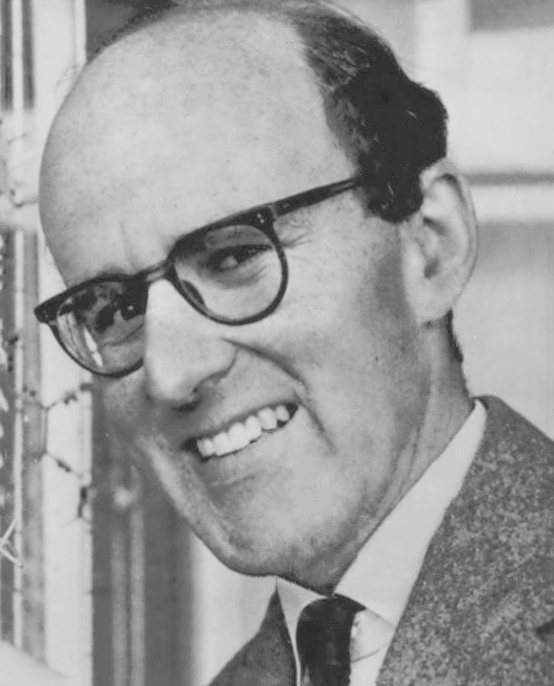
\includegraphics[width=0.30\linewidth]{images/book5/perutz.jpg}\hspace{0.04\linewidth}
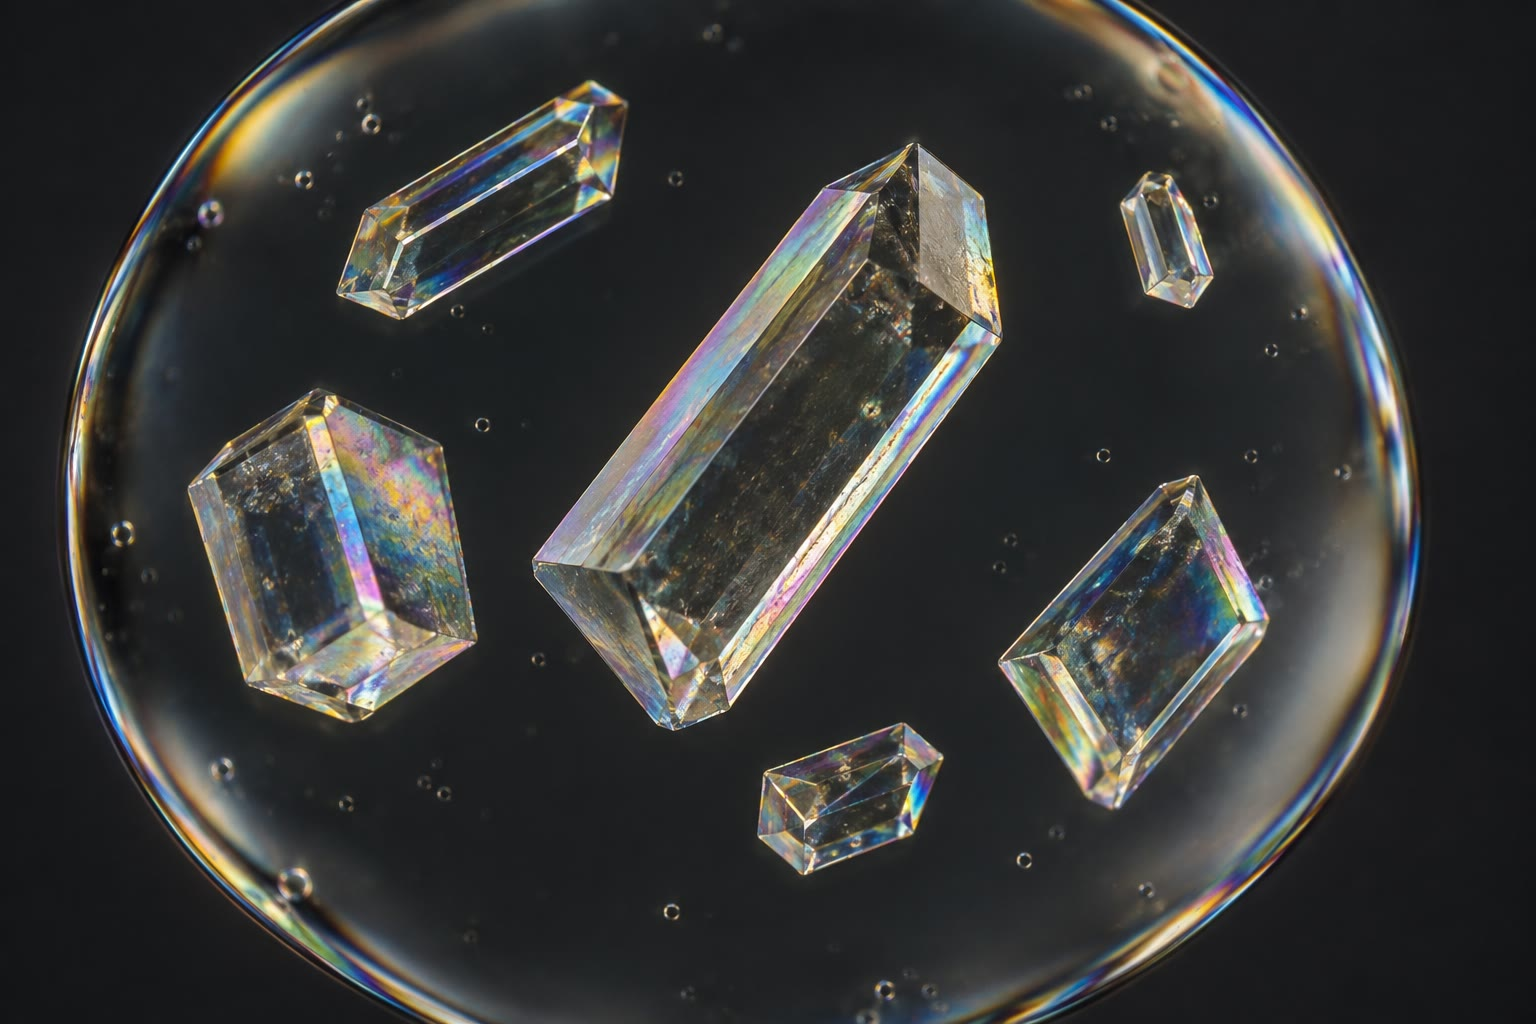
\includegraphics[width=0.30\linewidth]{images/book5/ai/b5-07-protein-crystals.jpg}\hspace{0.04\linewidth}
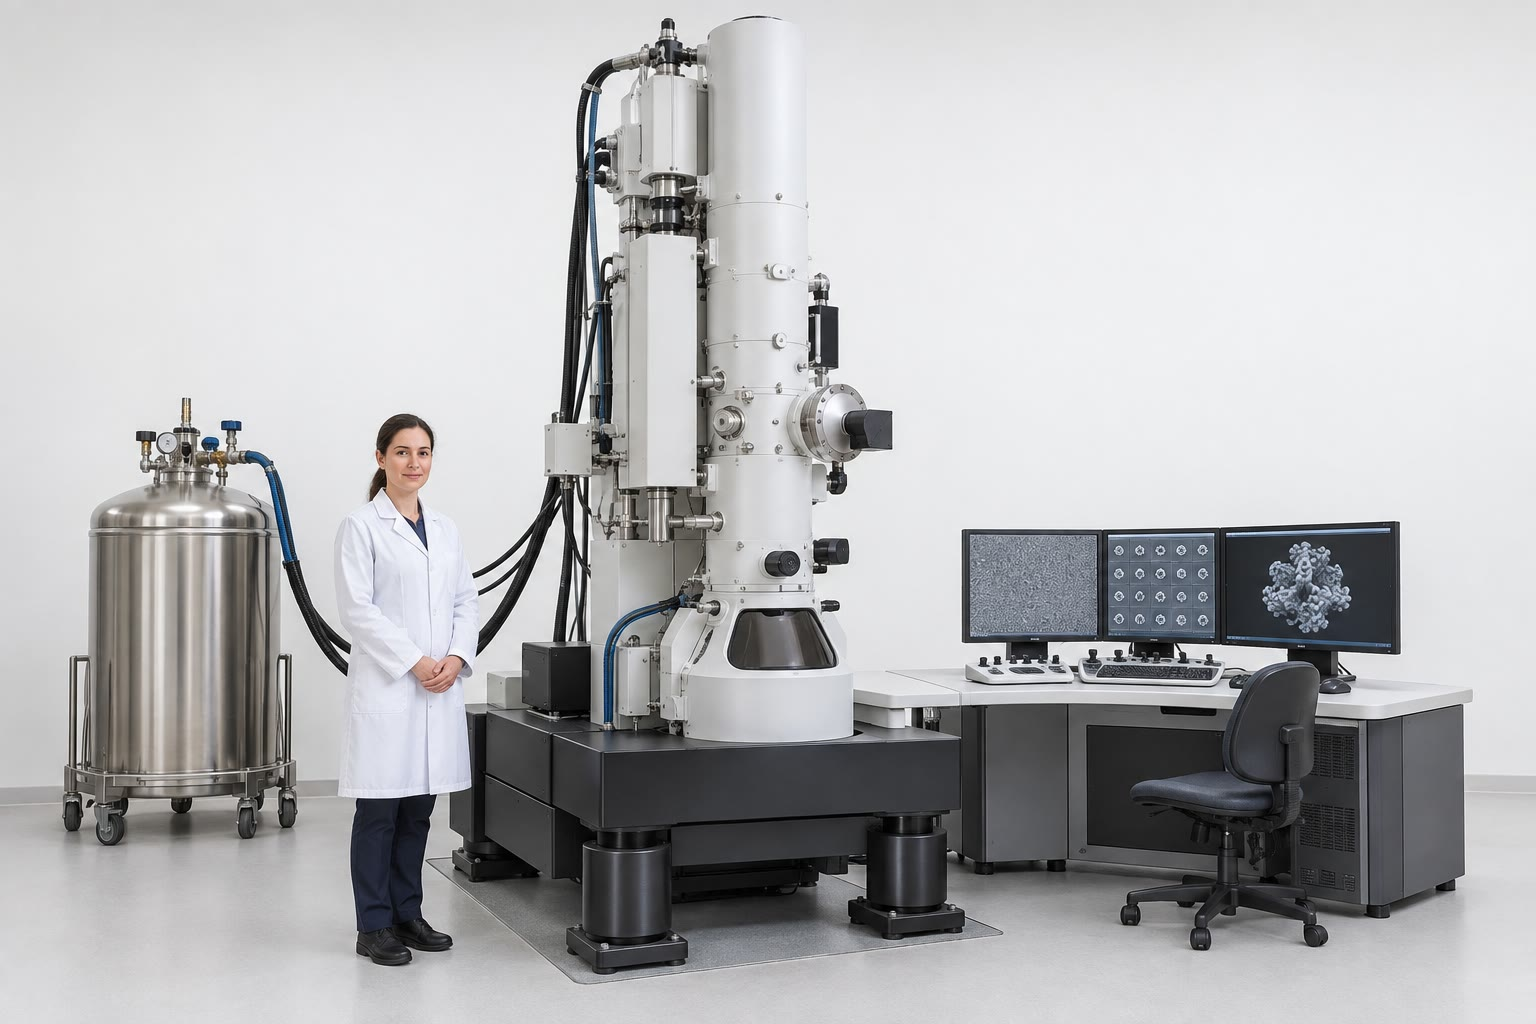
\includegraphics[width=0.30\linewidth]{images/book5/ai/b5-07-cryo-em.jpg}

{\small Max Perutz in 1962, het jaar van zijn Nobelprijs voor de
structuur van hemoglobine (Associated Press, publiek \omterm{def:b3:structural-biology:levels}{domein}). Midden:
eiwitkristallen in een hangende druppel, het vertrekpunt van de
kristallografie. Rechts: een cryo-elektronenmicroscoop, het instrument
dat kristallen overbodig maakte.}
\end{omfigure}

\begin{method}[Een structuur oplossen met kristallografie]\label{met:b3:structural-biology:crystallography}
\index{wet van Bragg}\index{faseprobleem}
(1) Zuiver milligrammen van het eiwit en beproef honderden
omstandigheden (neerslagmiddel, pH, zout) op kristallen; (2) bevries
een kristal razendsnel en verzamel diffractiebeelden bij een
synchrotron terwijl het in de bundel draait; (3) indexeer de vlekken om
de eenheidscel en de symmetrie te verkrijgen; de grootste hoek waarbij
nog vlekken worden gezien legt via de \omterm{met:b3:structural-biology:crystallography}{wet van Bragg} de \omterm{def:b3:structural-biology:methods}{resolutie} vast,
$d =
\lambda/(2\sin\theta)$; (4) los het \emph{faseprobleem} op --- de
detector registreert intensiteiten maar geen fasen --- met zware
atomen, met de anomale verstrooiing van selenium in selenomethionine,
of, voor een eiwit dat op een bekend eiwit lijkt, met moleculaire
vervanging, waarbij het bekende model in de cel wordt gelegd;
(5) bereken de elektronendichtheid, bouw de keten erin en verfijn het
model tegen de gegevens tot de afwijking ($R$-factor) klein is;
(6) valideer: meetkunde, uitschieters in de ramachandranplot, en de
overeenstemming met gegevens waartegen het model niet is verfijnd.
\end{method}

\begin{omfigure}
\begin{tikzpicture}[every node/.style={font=\scriptsize}, >=stealth]
  % crystal
  \draw[thick, fill=omDef!20] (0,0) -- (1.4,0) -- (1.9,0.6) -- (0.5,0.6) -- cycle; \draw[thick, fill=omDef!30] (0,0) -- (0.5,0.6) -- (0.5,1.6) -- (0,1.0) -- cycle; \draw[thick, fill=omDef!25] (0.5,0.6) -- (1.9,0.6) -- (1.9,1.6) -- (0.5,1.6) -- cycle;
  \node[below] at (0.95,-0.1) {kristal: $10^{12}$ moleculen in het gelid};
  % beam
  \draw[->, very thick, omThm] (-2.2,0.9) -- (-0.1,0.9); \node[above] at (-1.2,0.95) {röntgenstraling, $\lambda \approx \qty{0.1}{nm}$};
  % diffracted beams
  \foreach \a in {-25,-12,5,18,30} \draw[->, omThm, thick] (1.9,0.9) -- ++(\a:3.2);
  % detector
  \draw[thick] (5.2,-1.2) rectangle (5.6,3.0); \node[right, align=left] at (5.7,2.6) {detector: vlekken onder\\hoeken $\theta$, met\\intensiteiten $I$};
  \foreach \y in {-0.6,-0.1,0.6,1.2,1.9,2.4} \fill[black] (5.4,\y) circle (0.06);
  % arrow to density
  \draw[->, very thick] (7.4,0.9) -- (8.6,0.9) node[midway, above, align=center] {fasen\\teruggevonden};
  \node[right, align=left] at (8.7,1.4) {elektronendichtheid};
  \draw[omDef, thick] (8.8,0.4) .. controls (9.1,1.1) and (9.5,0.2) .. (9.8,0.8) .. controls (10.1,1.3) and (10.4,0.3) .. (10.7,0.9);
  \node[right, align=left] at (8.7,-0.4) {model erin gebouwd,\\verfijnd, gevalideerd};
  % Bragg
  \node[anchor=north west, align=left] at (-2.2,-0.7) {Bragg: $2d\sin\theta = \lambda$ ---\\de grootste waargenomen $\theta$ legt de resolutie $d$ vast};
\end{tikzpicture}

{\small Van kristal naar model. Het regelmatige rooster verstrooit de
röntgenstraling in afzonderlijke vlekken; de vlek onder de grootste
hoek legt de \omterm{def:b3:structural-biology:methods}{resolutie} vast; het terugvinden van de fasen maakt van de
intensiteiten een kaart van de elektronendichtheid, waarin de keten
wordt gebouwd.}
\end{omfigure}

\begin{remark}[De voorspelling is bij de methoden gekomen]\label{rem:b3:structural-biology:prediction}
Sinds 2020 wordt de structuur van een eiwit uit zijn sequentie
voorspeld met een nauwkeurigheid die vaak niet onderdoet voor een
experimentele structuur van \qty{0.3}{nm}
(\cref{ch:b3:bioinformatics}). De voorspelling is een hypothese over
een statische natieve toestand; de experimentele methoden blijven de
scheidsrechter en de enige bron van informatie over liganden,
conformatieveranderingen, complexen en de dynamica hieronder. Hun rollen
zijn veranderd --- een voorspeld model lost het faseprobleem op met
moleculaire vervanging en wijst aan welke experimenten de moeite waard
zijn --- en niet zozeer heeft de ene de andere vervangen.
\end{remark}

\section{Allosterie: hemoglobine als model}

\begin{definition}[Allosterie en coöperativiteit]\label{def:b3:structural-biology:allostery}
\index{allosterie}\index{coöperativiteit}\index{hillcoëfficiënt}\index{T-toestand}\index{R-toestand}
Een eiwit is \emph{allosterisch} wanneer de binding van een ligand op
de ene plaats de affiniteit van een andere plaats verandert, door een
conformatieverandering die door het molecuul wordt doorgegeven. Binden
de twee plaatsen hetzelfde ligand en is het effect positief, dan is de
binding \emph{coöperatief}: de fractionele verzadiging $Y$ stijgt met
de ligandconcentratie als een sigmoïde en niet als een hyperbool,
empirisch beschreven door de \emph{hillvergelijking}
$Y = [S]^{n_{H}}/(K^{n_{H}} +
[S]^{n_{H}})$ met een \emph{hillcoëfficiënt} $n_{H} > 1$ (hemoglobine:
$n_{H} \approx 2.8$ voor zijn vier plaatsen; myoglobine, met één
plaats: $n_{H} =
1$). Hemoglobine bestaat in twee quaternaire conformaties, de
\emph{T-toestand} (gespannen, lage affiniteit, bevoordeeld wanneer er
geen zuurstof is gebonden) en de \emph{R-toestand} (ontspannen, hoge
affiniteit), en schakelt als geheel tussen beide om; protonen,
kooldioxide en 2,3-bisfosfoglyceraat stabiliseren T en verlagen zo de
affiniteit --- het \omterm{prop:b3:structural-biology:mechanism}{Bohr-effect}, waardoor werkend weefsel, zuur en warm,
meer zuurstof uit het bloed haalt.
\end{definition}

\begin{theorem}[Het model van Monod--Wyman--Changeux]\label{thm:b3:structural-biology:mwc}
\index{model van Monod--Wyman--Changeux}\index{gelijktijdig model}
Laat een eiwit met $n$ gelijke plaatsen in twee conformaties bestaan,
$T$ en $R$, in evenwicht $L = [T_{0}]/[R_{0}]$ zonder ligand, waarbij
elke plaats van $R$ het ligand bindt met dissociatieconstante $K_{R}$
en elke plaats van $T$ met $K_{T}$, met $c = K_{R}/K_{T} < 1$. Alle
plaatsen van een molecuul schakelen samen om (de overgang is
\emph{gelijktijdig}). Dan is met $\alpha = [S]/K_{R}$ de fractionele
verzadiging
\[
Y = \frac{\alpha(1+\alpha)^{n-1} + Lc\alpha(1+c\alpha)^{n-1}}
{(1+\alpha)^{n} + L(1+c\alpha)^{n}},
\]
en is het deel van de moleculen in de $R$-toestand $\bar R =
(1+\alpha)^{n}/\bigl[(1+\alpha)^{n} + L(1+c\alpha)^{n}\bigr]$. Voor $L
\gg 1$ en $c \ll 1$ is de curve sigmoïde: de eerste liganden binden aan
de schaarse $R$-moleculen met hoge affiniteit en doen het evenwicht
kantelen, zodat de binding meer $R$ werft en de affiniteit van de
overige plaatsen stijgt --- \omterm{def:b3:structural-biology:allostery}{coöperativiteit} zonder enige rechtstreekse
wisselwerking tussen de plaatsen.
\end{theorem}
\begin{proof}
De soort met $i$ gebonden liganden in de $R$-vorm heeft concentratie
$[R_{0}]\binom{n}{i}\alpha^{i}$ (elk van de $\binom{n}{i}$ keuzen van
bezette plaatsen draagt $([S]/K_{R})^{i}$ bij volgens de wet van de
massawerking), en in de $T$-vorm $[T_{0}]\binom{n}{i}(c\alpha)^{i}$,
omdat $[S]/K_{T} = c\alpha$. Sommeren over $i$ met het binomium geeft
als totaal eiwit $[R_{0}]\bigl[(1+\alpha)^{n} + L(1+c\alpha)^{n}\bigr]$
en als totaal gebonden ligand $[R_{0}]\sum_{i} i\binom{n}{i}\bigl[
\alpha^{i} + L(c\alpha)^{i}\bigr] = [R_{0}]\,n\bigl[\alpha(1+\alpha)^{n-1}
+ Lc\alpha(1+c\alpha)^{n-1}\bigr]$, met $\sum_{i} i\binom{n}{i}x^{i} =
nx(1+x)^{n-1}$. Het gebonden ligand delen door $n$ maal het totale
eiwit geeft $Y$; het $R$-deel is de som van de $R$-termen gedeeld door
het totaal. Is $\alpha$ klein, dan overheersen de $T$-termen de noemer
(omdat $L \gg 1$) en is $Y \approx c\alpha$, de lage affiniteit van
$T$; is $\alpha$ groot genoeg dat
$(1+\alpha)^{n} > L(1+c\alpha)^{n}$, dan nemen de $R$-termen het over
en is de affiniteit $K_{R}$: de omschakeling tussen beide regimes is de
sigmoïde.
\end{proof}

\begin{example}[Hemoglobine in getallen]\label{ex:b3:structural-biology:hb-numbers}
Neem $n = 4$, $K_{R} = \qty{1}{mmHg}$, $c = 0.01$ (dus $K_{T} =
\qty{100}{mmHg}$) en $L = 3\times 10^{5}$. Bij de partiële druk van
zuurstof in arterieel bloed, \qty{100}{mmHg}, is $\alpha = 100$ en $Y =
0.97$; bij \qty{40}{mmHg}, de veneuze waarde in rust, is $Y = 0.78$;
bij \qty{26}{mmHg} is $Y = 0.52$ --- het model geeft de
halfverzadigingsdruk van \qty{26}{mmHg} weer; bij \qty{20}{mmHg}, in
een werkende spier, is $Y = 0.35$. Een niet-coöperatieve drager met
dezelfde halfverzadigingsdruk zou $100/126 = 0.79$ in de longen en
$20/46 = 0.43$ in de spier geven, en dus $0.36$ van zijn capaciteit
lossen waar hemoglobine $0.62$ lost. De \omterm{def:b3:structural-biology:allostery}{coöperativiteit} maakt een
drager die bij de ene druk volledig laadt en bij een druk die maar vijf
keer lager is grotendeels lost.
\end{example}

\begin{omfigure}
\begin{tikzpicture}
\begin{axis}[
  width=0.7\linewidth, height=5.8cm,
  axis x line=bottom, axis y line=left,
  xmin=0, xmax=120, ymin=0, ymax=1.05,
  xlabel={partiële zuurstofdruk (mmHg)}, ylabel={verzadiging $Y$},
  xlabel style={font=\small, at={(axis description cs:0.5,-0.12)}, anchor=north},
  ylabel style={font=\small},
  tick label style={font=\small}, xtick={0,20,40,60,80,100,120}, ytick={0,0.5,1},
  clip=false,
]
\addplot[very thick, omThm, domain=0.1:120, samples=120] {(x*(1+x)^3 + 300000*0.01*x*(1+0.01*x)^3)/((1+x)^4 + 300000*(1+0.01*x)^4)};
\addplot[very thick, omDef, domain=0:120, samples=60] {x/(x+26)};
\addplot[dashed, gray] coordinates {(26,0) (26,0.52)}; \addplot[dashed, gray] coordinates {(0,0.52) (26,0.52)};
\draw[gray, dashed] (axis cs:20,0) -- (axis cs:20,0.35); \draw[gray, dashed] (axis cs:100,0) -- (axis cs:100,0.97);
\node[font=\scriptsize, omThm, anchor=north west] at (axis cs:50,0.15) {hemoglobine (MWC, $n = 4$, $L = 3\times 10^{5}$, $c = 0.01$)};
\node[font=\scriptsize, omDef, anchor=north east] at (axis cs:118,0.72) {één plaats, dezelfde $P_{50}$};
\node[font=\scriptsize, anchor=south] at (axis cs:20,1.0) {spier}; \node[font=\scriptsize, anchor=south] at (axis cs:100,1.0) {long};
\end{axis}
\end{tikzpicture}

{\small Zuurstofverzadiging van hemoglobine, berekend met de
vergelijking van Monod--Wyman--Changeux met de parameters van het
voorbeeld (rood), tegenover een drager met één plaats en dezelfde
halfverzadigingsdruk (blauw). Tussen long en werkende spier lost de
coöperatieve drager bijna tweemaal zoveel.}
\end{omfigure}

\begin{proposition}[Het mechanisme van de omschakeling]\label{prop:b3:structural-biology:mechanism}
\index{Bohr-effect}\index{2,3-bisfosfoglyceraat}
In deoxyhemoglobine ligt het ijzer iets buiten het vlak van de heem,
naar het proximale histidine getrokken, en is de heem gewelfd. Het
binden van zuurstof vlakt de heem af en trekt het ijzer, en daarmee het
histidine en de helix waartoe het behoort, ongeveer \qty{0.06}{nm} naar
de heem toe; die verschuiving wordt versterkt aan het raakvlak tussen
de dimeren $\alpha_{1}\beta_{1}$ en $\alpha_{2}\beta_{2}$, die over
\qty{15}{\degree} draaien en de zoutbruggen verbreken die de
\omterm{def:b3:structural-biology:allostery}{T-toestand} vasthouden. De effectoren werken op diezelfde bruggen:
protonen binden aan histidines waarvan de bruggen alleen in T bestaan
(het \omterm{prop:b3:structural-biology:mechanism}{Bohr-effect}), kooldioxide vormt carbamaten met de aminotermini die
T stabiliseren, en 2,3-bisfosfoglyceraat, een sterk negatief klein
molecuul, zit in de centrale holte tussen de $\beta$-ketens, die alleen
in T wijd genoeg is. Foetaal hemoglobine, met $\gamma$-ketens die het
minder goed binden, heeft een hogere affiniteit dan dat van de moeder
en trekt zuurstof over de placenta.
\end{proposition}

\section{Eiwitten in beweging}

\begin{definition}[Wanorde en dynamica]\label{def:b3:structural-biology:disorder}
\index{intrinsiek wanordelijk eiwit}\index{conformatie-ensemble}\index{biomoleculair condensaat}
Een \emph{intrinsiek wanordelijk} gebied heeft op zichzelf geen
stabiele \omterm{def:b3:structural-biology:levels}{vouwing} en bestaat als een ensemble van snel in elkaar
overgaande conformaties, en vouwt zich vaak pas wanneer het zijn
partner ontmoet; ongeveer een derde van de menselijke eiwitten draagt
een wanordelijk gebied van meer dan dertig residuen, en zij zijn
verrijkt in signalering en regulatie, waar een buigzaam segment op vele
plaatsen kan worden gefosforyleerd, achtereenvolgens verscheidene
partners kan binden en als verbindingsstuk kan dienen. Ook gevouwen
eiwitten bewegen: zijketens draaien in picoseconden, lussen gaan in
nanoseconden tot microseconden open, \omterm{def:b3:structural-biology:levels}{domeinen} scharnieren in
microseconden tot milliseconden, en de katalytische cyclus van een
enzym is eerder een choreografie van zulke bewegingen dan een statisch
slot met sleutel. Een kristalstructuur is één momentopname van een
\emph{conformatie-ensemble}; NMR en moleculaire simulatie zien de rest.
Meerwaardige wanordelijke eiwitten en RNA's kunnen zich ook uit het
cytoplasma ontmengen tot vloeibare druppels --- \emph{biomoleculaire
condensaten} zoals nucleoli, stressgranules en P-lichaampjes --- die
reacties zonder membraan concentreren, en waarvan de veroudering tot
vaste klonters een van de wegen naar de amyloïdziekten is.
\end{definition}

\begin{remark}[Structuur en functie]\label{rem:b3:structural-biology:sf}
De les van zestig jaar structuren is dubbel. Een \omterm{def:b3:structural-biology:levels}{vouwing} is een
oplossing voor een natuurkundig probleem --- dit binden, dat
katalyseren, een signaal over vier nanometer doorgeven --- en de
structuur kennen maakt het mechanisme vaak meteen duidelijk, zoals bij
het ijzer van de heem en bij de door zuurstof aangedreven draaiing van
de dimeren van hemoglobine. En een \omterm{def:b3:structural-biology:levels}{vouwing} is een historisch voorwerp:
dezelfde paar honderd bouwplannen, bijgeschaafd, verdubbeld en
versmolten, bedienen de hele verscheidenheid aan eiwitfuncties, zodat
de structuur van een eiwit uit een bacterie vaak vertelt hoe de
menselijke neef werkt.
\end{remark}

\section{Opgaven}

\begin{exercise}[$\star$]\label{exo:b3:structural-biology:1}
Definieer de vier structuurniveaus van een eiwit en geef van elk het
voorbeeld in hemoglobine.
\end{exercise}

\begin{exercise}[$\star$]\label{exo:b3:structural-biology:2}
Een $\alpha$-helix bevat $36$ residuen. Hoe lang is zij, hoeveel
windingen maakt zij, en hoeveel waterstofbruggen van de ruggengraat
houden haar bijeen (het carbonyl van elk residu bindt aan het amide
vier residuen verder)?
\end{exercise}

\begin{exercise}[$\star$]\label{exo:b3:structural-biology:3}
Wat toonde Anfinsens hervouwing van ribonuclease aan, en waarom was het
belangrijk het experiment zonder enig celbestanddeel uit te voeren?
\end{exercise}

\begin{exercise}[$\star$]\label{exo:b3:structural-biology:4}
Rangschik kristallografie, NMR en \omterm{def:b3:structural-biology:methods}{cryo-elektronenmicroscopie} naar de
grootte van het eiwit dat elk het best aankan, en zeg welke informatie
over beweging geeft.
\end{exercise}

\begin{exercise}[$\star\star$]\label{exo:b3:structural-biology:5}
Doe de telling van Levinthal opnieuw voor een eiwit van $150$ residuen
met $k = 2$, en voor een peptide van $20$ residuen met $k = 3$. Voor
welk van de twee is een willekeurige zoektocht binnen een seconde
denkbaar bij $10^{12}$ pogingen per seconde?
\end{exercise}

\begin{exercise}[$\star\star$]\label{exo:b3:structural-biology:6}
Bereken met de MWC-vergelijking bij $n = 2$, $L = 100$, $c = 0.01$ de
waarde van $Y$ bij $\alpha = 1$, $10$ en $100$, en vergelijk met één
plaats met dissociatieconstante $K_{R}$ ($Y = \alpha/(1+\alpha)$). Waar
blijkt de \omterm{def:b3:structural-biology:allostery}{coöperativiteit}?
\end{exercise}

\begin{exercise}[$\star\star$]\label{exo:b3:structural-biology:7}
Leg met het MWC-model uit waarom 2,3-bisfosfoglyceraat de
zuurstofaffiniteit van hemoglobine verlaagt, welke parameter van het
model het verandert, en waarom bewaard bloed, dat de stof verliest, bij
transfusie slecht zuurstof afgeeft.
\end{exercise}

\begin{exercise}[$\star\star$]\label{exo:b3:structural-biology:8}
Een kristal diffracteert tot een grootste hoek $\theta = \qty{15}{\degree}$
met röntgenstraling van golflengte \qty{0.1}{nm}. Wat is de \omterm{def:b3:structural-biology:methods}{resolutie}?
Welke kenmerken van het eiwit zullen zichtbaar zijn? Welke hoek zou
voor \qty{0.12}{nm} nodig zijn?
\end{exercise}

\begin{exercise}[$\star\star$]\label{exo:b3:structural-biology:9}
Een mutatie vervangt een begraven leucine door een lysine. Voorspel het
effect op de stabiliteit met
\cref{prop:b3:structural-biology:forces}, en leg uit waarom dezelfde
vervanging aan het oppervlak onschadelijk zou zijn. Leg daarna uit
waarom een eiwit met $\Delta G_{\text{fold}} =
\qty{-30}{kJ/mol}$ niet ``zeer stabiel'' is, hoewel het getal groot
lijkt.
\end{exercise}

\begin{exercise}[$\star\star\star$]\label{exo:b3:structural-biology:10}
Leid het deel van de moleculen in de $R$-toestand, $\bar R$, af uit de
soorten die in het bewijs van \cref{thm:b3:structural-biology:mwc}
worden geteld, en laat zien dat voor $c \to 0$ de ligandconcentratie
waarbij de helft van de moleculen in $R$ is voldoet aan
$(1+\alpha)^{n} = L$. Bereken deze $\alpha$ voor de parameters van
hemoglobine en vergelijk met $P_{50}$.
\end{exercise}

\begin{exercise}[$\star\star\star$]\label{exo:b3:structural-biology:11}
\omterm{def:b3:structural-biology:amyloid}{Prionen} dragen een vorm over. Leg uit waarom de hypothese ``alleen
eiwit'' op weerstand stuitte, welk experiment haar zou weerleggen, en
welke aanwijzingen (bestandheid van de besmettelijkheid tegen nucleasen
en ultraviolet licht, gevoeligheid voor eiwitdenaturerende middelen,
synthetische \omterm{def:b3:structural-biology:amyloid}{prionen}) haar steunen. Waarom heeft een \omterm{def:b3:structural-biology:amyloid}{prion} een kiem
nodig?
\end{exercise}

\begin{exercise}[$\star\star\star$]\label{exo:b3:structural-biology:12}
Een eiwitfamilie heeft haar \omterm{def:b3:structural-biology:levels}{vouwing} behouden terwijl haar sequenties
tot \qty{15}{\%} identiteit uiteen zijn gegroeid. Leg uit waarom de
structuur beter bewaard blijft dan de sequentie, welke soort residuen
de bewaarde zijn, en hoe dit zowel door profielmethoden
(\cref{ch:b3:bioinformatics}) als bij het ontwerpen van nieuwe eiwitten
wordt benut.
\end{exercise}

\section{Vraagstuk: de vouwing van een globine}

\begin{problem}[{Weekendvraagstuk --- de helices van een globine
gemeten, zijn vouwing tegen Levinthal in de tijd gezet, zijn
zuurstofbinding berekend met het tweetoestandsmodel, en zijn structuur
opgelost uit een kristal, met als besluit het verzadigingsverschil
tussen long en spier, de tijd van Levinthal en de resolutie van de
kaart}]
\label{pb:b3:structural-biology:1}
Gegevens: een globineketen van $150$ residuen, gemiddelde residumassa
\qty{110}{Da}, met \qty{75}{\%} van de residuen in acht
$\alpha$-helices; helixstijging \qty{0.15}{nm} per residu, $3.6$
residuen per winding. Partieel soortelijk volume van eiwit
\qty{0.73}{cm^3/g}. MWC-parameters voor hemoglobine: $n = 4$,
$K_{R} = \qty{1}{mmHg}$, $c = 0.01$, $L = 3\times 10^{5}$.
Röntgengolflengte \qty{0.1}{nm}; eenheidscel een kubus met ribbe
\qty{6}{nm}; kristal een kubus met ribbe \qty{100}{\micro m}.

\medskip
\noindent\textbf{Deel I --- Anatomie van een keten.}
\begin{enumerate}
  \item Hoeveel residuen zitten er in helices? Welke totale helixlengte
        is dat, en hoeveel windingen?
  \item Hoeveel waterstofbruggen van de ruggengraat bevatten de
        helices, geteld als één per residu voorbij de eerste vier van
        elke helix?
  \item Bereken de massa van de keten en haar volume uit het partieel
        soortelijk volume, en de straal van een bol met dat volume.
  \item De gestrekte keten zou \qty{0.36}{nm} per residu lang zijn.
        Vergelijk haar lengte met de diameter van de bol: met welke
        factor comprimeert het vouwen de keten?
  \item De acht helices tellen gemiddeld $14$ residuen. Welk deel van
        de gestrekte lengte is helicaal als de residuen achter elkaar
        zouden liggen, en hoezeer verkort de helix haar?
  \item Een globine begraaft ongeveer $40$ apolaire zijketens in zijn
        kern. Schat met \qty{4}{kJ/mol} hydrofobe stabilisatie per
        begraven zijketen en een kost aan conformatie-entropie van
        \qty{0.9}{kJ/mol} per residu bij het vouwen (alle $150$) de
        netto $\Delta G$ van het vouwen, en vergelijk met het bereik in
        \cref{prop:b3:structural-biology:forces}.
\end{enumerate}

\medskip
\noindent\textbf{Deel II --- De \omterm{def:b3:structural-biology:levels}{vouwing} vinden.}
\begin{enumerate}[resume]
  \item Bereken de telling van Levinthal voor $150$ residuen met
        $k = 3$ en de tijd om haar te doorlopen bij $10^{12}$ per
        seconde.
  \item Het globine vouwt zich in \qty{10}{ms}. Hoeveel conformaties
        kan het hoogstens hebben bezocht? Welk deel van de telling is
        dat?
  \item Stel in plaats daarvan dat elke helix zich onafhankelijk in
        \qty{1}{\micro s} vormt, en dat de acht gevormde helices hun
        pakking daarna zoeken tussen $8!$ volgordes die bij $10^{6}$
        per seconde worden bemonsterd. Schat de vouwtijd. Is dit een
        trechter?
  \item Een \omterm{def:b3:structural-biology:chaperones}{chaperonine} sluit een keten \qty{10}{s} per cyclus op en
        laat haar met kans $0.3$ per cyclus gevouwen los. Wat is het
        verwachte aantal cycli, en de verwachte tijd, om een lastig
        substraat te vouwen? Welk deel is na een minuut nog ongevouwen?
  \item Een destabiliserende mutatie verhoogt het ongevouwen deel bij
        \qty{37}{\celsius} van $10^{-4}$ naar $10^{-2}$. Hoeveel is met
        $\Delta G =
        -RT\ln(K)$ en $K = [\text{gevouwen}]/[\text{ongevouwen}]$
        $\Delta G_{\text{fold}}$ veranderd?
  \item Leg met de noodzaak van een kiem uit waarom honderd keer meer
        ongevouwen eiwit het verschil kan zijn tussen gezondheid en een
        amyloïdziekte.
\end{enumerate}

\medskip
\noindent\textbf{Deel III --- Zuurstof binden.}
\begin{enumerate}[resume]
  \item Bereken $Y$ met de MWC-vergelijking bij $\alpha = 100$ (long)
        en $\alpha = 20$ (werkende spier).
  \item Bereken het deel van de moleculen in de $R$-toestand bij die
        twee drukken.
  \item Hoeveel van de geladen zuurstof wordt tussen long en spier
        gelost? Vergelijk met een drager met één plaats en een
        halfverzadigingsdruk van \qty{26}{mmHg}.
  \item Bloed draagt \qty{150}{g} hemoglobine per liter, en elke gram
        bindt \qty{1.34}{mL} zuurstof. Hoeveel milliliter zuurstof per
        liter levert hemoglobine aan de spier volgens vraag 15? Een
        lichaam in rust verbruikt \qty{250}{mL/min}: welke
        bloedstroom vergt dat in rust (lossen van $0.97$ naar $0.78$)?
  \item Bisfosfoglyceraat verhoogt $L$ tot $3\times 10^{6}$. Herbereken
        $Y$ bij $\alpha = 40$ en zeg wat dit met de levering in rust
        doet.
  \item Foetaal hemoglobine heeft in feite $L = 3\times 10^{4}$.
        Bereken zijn $Y$ bij de placentadruk van \qty{30}{mmHg},
        vergelijk met dat van de moeder, en verklaar de overdracht.
\end{enumerate}

\medskip
\noindent\textbf{Deel IV --- Het zien.}
\begin{enumerate}[resume]
  \item Hoeveel eenheidscellen bevat het kristal? Hoeveel moleculen
        diffracteren samen als elke cel vier globineketens bevat?
  \item Er worden vlekken gezien tot $\theta = \qty{14.5}{\degree}$.
        Wat is de \omterm{def:b3:structural-biology:methods}{resolutie}, en zullen de zijketens worden geplaatst?
  \item Welke hoek zou \qty{0.15}{nm} geven? Waarom diffracteert een
        slecht geordend kristal alleen tot kleine hoeken?
  \item In de \omterm{def:b3:structural-biology:methods}{cryo-elektronenmicroscopie} groeit het signaal van het
        gemiddelde beeld als de wortel uit het aantal deeltjes. Als
        \num{10000} deeltjes \qty{0.6}{nm} geven, en de \omterm{def:b3:structural-biology:methods}{resolutie}
        verbetert als het omgekeerde van het signaal, hoeveel deeltjes
        geven dan \qty{0.3}{nm}?
  \item De \omterm{def:b3:structural-biology:methods}{cryo-elektronenmicroscopie} heeft geen kristal nodig. Noem
        twee soorten eiwitten of complexen waarvoor dit beslist of er
        überhaupt een structuur te verkrijgen is, en leg uit waarom.
  \item Een voorspeld model van het globine wijkt over de ruggengraat
        gemiddeld \qty{0.1}{nm} van de kristalstructuur af. Noem twee
        dingen die de voorspelling niet kan leveren en het kristal wel.
  \item Vat samen: het lossen tussen long en spier (vraag~15), de tijd
        van Levinthal voor $150$ residuen (vraag~7), en de \omterm{def:b3:structural-biology:methods}{resolutie} van
        de kaart (vraag~20).
\end{enumerate}
\end{problem}
